\documentclass{beamer}
\usetheme{Darmstadt}
\usepackage{CJKutf8}

\usepackage[utf8]{inputenc}
\usepackage[OT1, T2A]{fontenc}
\usepackage{fontspec}
\usepackage[normalem]{ulem}

\usepackage{graphicx}
\usepackage{tikz}
\usetikzlibrary{quantikz}
\usepackage{braket}

\usepackage{xcolor}
\usepackage{pgfplots}
\usepackage{tikz}

\begin{document}
    \begin{frame}{Quantumizing S-DES}
        \begin{itemize}
            \item Most parts are permutations or compressions; no problems here.
            \item Two parts poses a challenge:
        \end{itemize}
        \begin{enumerate}
            \item S-Boxes
            \item Expansion
        \end{enumerate}
    \end{frame}

    \begin{frame}{Dealing with Expansions}
        \begin{itemize}
            \item Due to \href{https://en.wikipedia.org/wiki/No-cloning_theorem}{No-cloning theorem}, directly copying a qubit is not possible.
            \item Use XOR(CNOT) operation to copy the information.
        \end{itemize}
    \end{frame}

    \begin{frame}{Dealing with S-boxes}
        Consists of Lookup tables: Not ideal for quantum computing
        \begin{figure}[h]
            \centering
            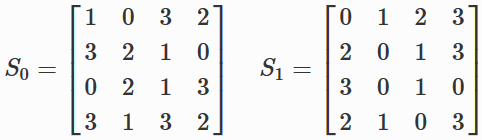
\includegraphics[width=0.5\textwidth]{./Images/sbox.png}
        \end{figure}
    \end{frame}

    \begin{frame}{Dealing with S-boxes: Quine-McCluskey Method}
        \begin{itemize}
            \item Break the S-Boxes into fundamental and/or/not-gates
            \item Letting the input bits into S-Boxes $ABCD$:
            \begin{itemize}
                \item S0 bit 1: $AB'C'+A'B'C+BCD'+ABD+BC'D$
                \item S0 bit 2: $AD'+B'D'+A'BC+ABC'$
                \item S1 bit 1: $AB'C'+ACD+A'CD'+A'BD'$
                \item S2 bit 2: $B'C'D+AB'C+BCD+BC'D'$
            \end{itemize}
            \item Directly calculating this would cause too many ancilla bits to use, i.e. for each and/or operation, one ancilla bit is required.
        \end{itemize}
    \end{frame}


    \begin{frame}{Dealing with S-boxes: The Brute-force Method}
    For each possibility in the S-box input, use a circuit similar to this:
    \begin{center}
    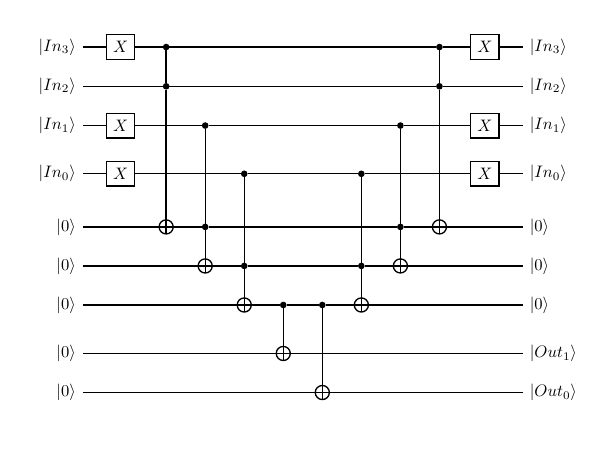
\begin{tikzpicture}
    \node[scale=0.6] {
    \begin{quantikz}
    \lstick{$\ket{In_3}$} & \gate{X} & \ctrl{1} & \qw & \qw & \qw & \qw & \qw & \qw & \ctrl{1} & \gate{X} & \qw  \rstick{$\ket{In_3}$} \\
    \lstick{$\ket{In_2}$} & \qw & \ctrl{3} & \qw & \qw & \qw & \qw & \qw & \qw & \ctrl{3} & \qw & \qw \rstick{$\ket{In_2}$} \\
    \lstick{$\ket{In_1}$} & \gate{X} & \qw & \ctrl{3} & \qw & \qw & \qw & \qw & \ctrl{3} & \qw & \gate{X} & \qw \rstick{$\ket{In_1}$} \\
    \lstick{$\ket{In_0}$} & \gate{X} & \qw & \qw & \ctrl{3} & \qw & \qw & \ctrl{3} & \qw & \qw & \gate{X} & \qw \rstick{$\ket{In_0}$} \\[0.2cm]
    \lstick{$\ket{0}$} & \qw & \targ{} & \ctrl{1} & \qw & \qw & \qw & \qw & \ctrl{1} & \targ{} & \qw & \qw \rstick{$\ket{0}$} \\
    \lstick{$\ket{0}$} & \qw & \qw & \targ{} & \ctrl{1} & \qw & \qw & \ctrl{1} & \targ{} & \qw & \qw & \qw \rstick{$\ket{0}$} \\
    \lstick{$\ket{0}$} & \qw & \qw & \qw & \targ{} & \ctrl{1} & \ctrl{2} & \targ{} & \qw & \qw & \qw & \qw \rstick{$\ket{0}$} \\[0.2cm]
    \lstick{$\ket{0}$} & \qw & \qw & \qw & \qw & \targ{} & \qw & \qw & \qw & \qw & \qw & \qw \rstick{$\ket{Out_1}$} \\
    \lstick{$\ket{0}$} & \qw & \qw & \qw & \qw & \qw & \targ{} & \qw & \qw & \qw & \qw & \qw \rstick{$\ket{Out_0}$}\\
    \end{quantikz}
    };
    \end{tikzpicture}
    \end{center}
    ...which requires 3 ancilla qubits.
    \end{frame}

    \begin{frame}{Dealing with S-boxes: The Brute-force Method}
    Thanks to the Microsoft Q\# library, we don't need that much ancilla qubits.
    \begin{center}
    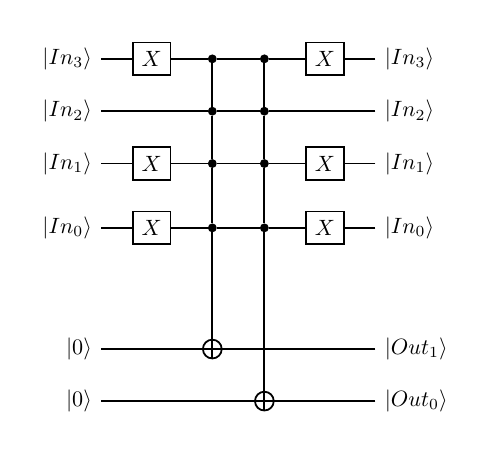
\begin{tikzpicture}
    \node[scale=0.8] {
    \begin{quantikz}
    \lstick{$\ket{In_3}$} & \gate{X} & \ctrl{1} & \ctrl{1} & \gate{X} & \qw \rstick{$\ket{In_3}$} \\
    \lstick{$\ket{In_2}$} & \qw & \ctrl{1} & \ctrl{1} & \qw & \qw \rstick{$\ket{In_2}$} \\
    \lstick{$\ket{In_1}$} & \gate{X} & \ctrl{1} & \ctrl{1} & \gate{X} & \qw \rstick{$\ket{In_1}$} \\
    \lstick{$\ket{In_0}$} & \gate{X} & \ctrl{1} & \ctrl{2} & \gate{X} & \qw \rstick{$\ket{In_0}$} \\[1cm]
    \lstick{$\ket{0}$} & \qw & \targ & \qw & \qw & \qw & \qw \rstick{$\ket{Out_1}$} \\
    \lstick{$\ket{0}$} & \qw & \qw & \targ & \qw & \qw & \qw  \rstick{$\ket{Out_0}$}
    \end{quantikz}
    };
    \end{tikzpicture}
    \end{center}
    No (explicit) ancilla qubits are required!
    \end{frame}

    \begin{frame}{Dealing with S-boxes: Combining the two methods?}
        \begin{itemize}
            \item Still a hypothetical yet.
            \item The structure of Quine-McCluskey simplified S-Box is similar to Brute-force
            \item The number of terms may decrease significantly, and one ancilla bit can definitely be removed.
            \item Needs further testing...
        \end{itemize}
    \end{frame}
\end{document}